\section{Thiết lập thực nghiệm}\label{sec:thiet-lap}

\subsection{Quy trình thực nghiệm}
Hình~\ref{fig:pipeline} tóm tắt quy trình một lượt thực nghiệm. Phía trên là mô hình thật, chỉ bước chấm điểm được truy cập; phía dưới là những gì phương pháp được thấy: dữ liệu, skeleton đã làm hỏng và số cạnh hỏng khai báo.

\begin{figure}[H]
\centering
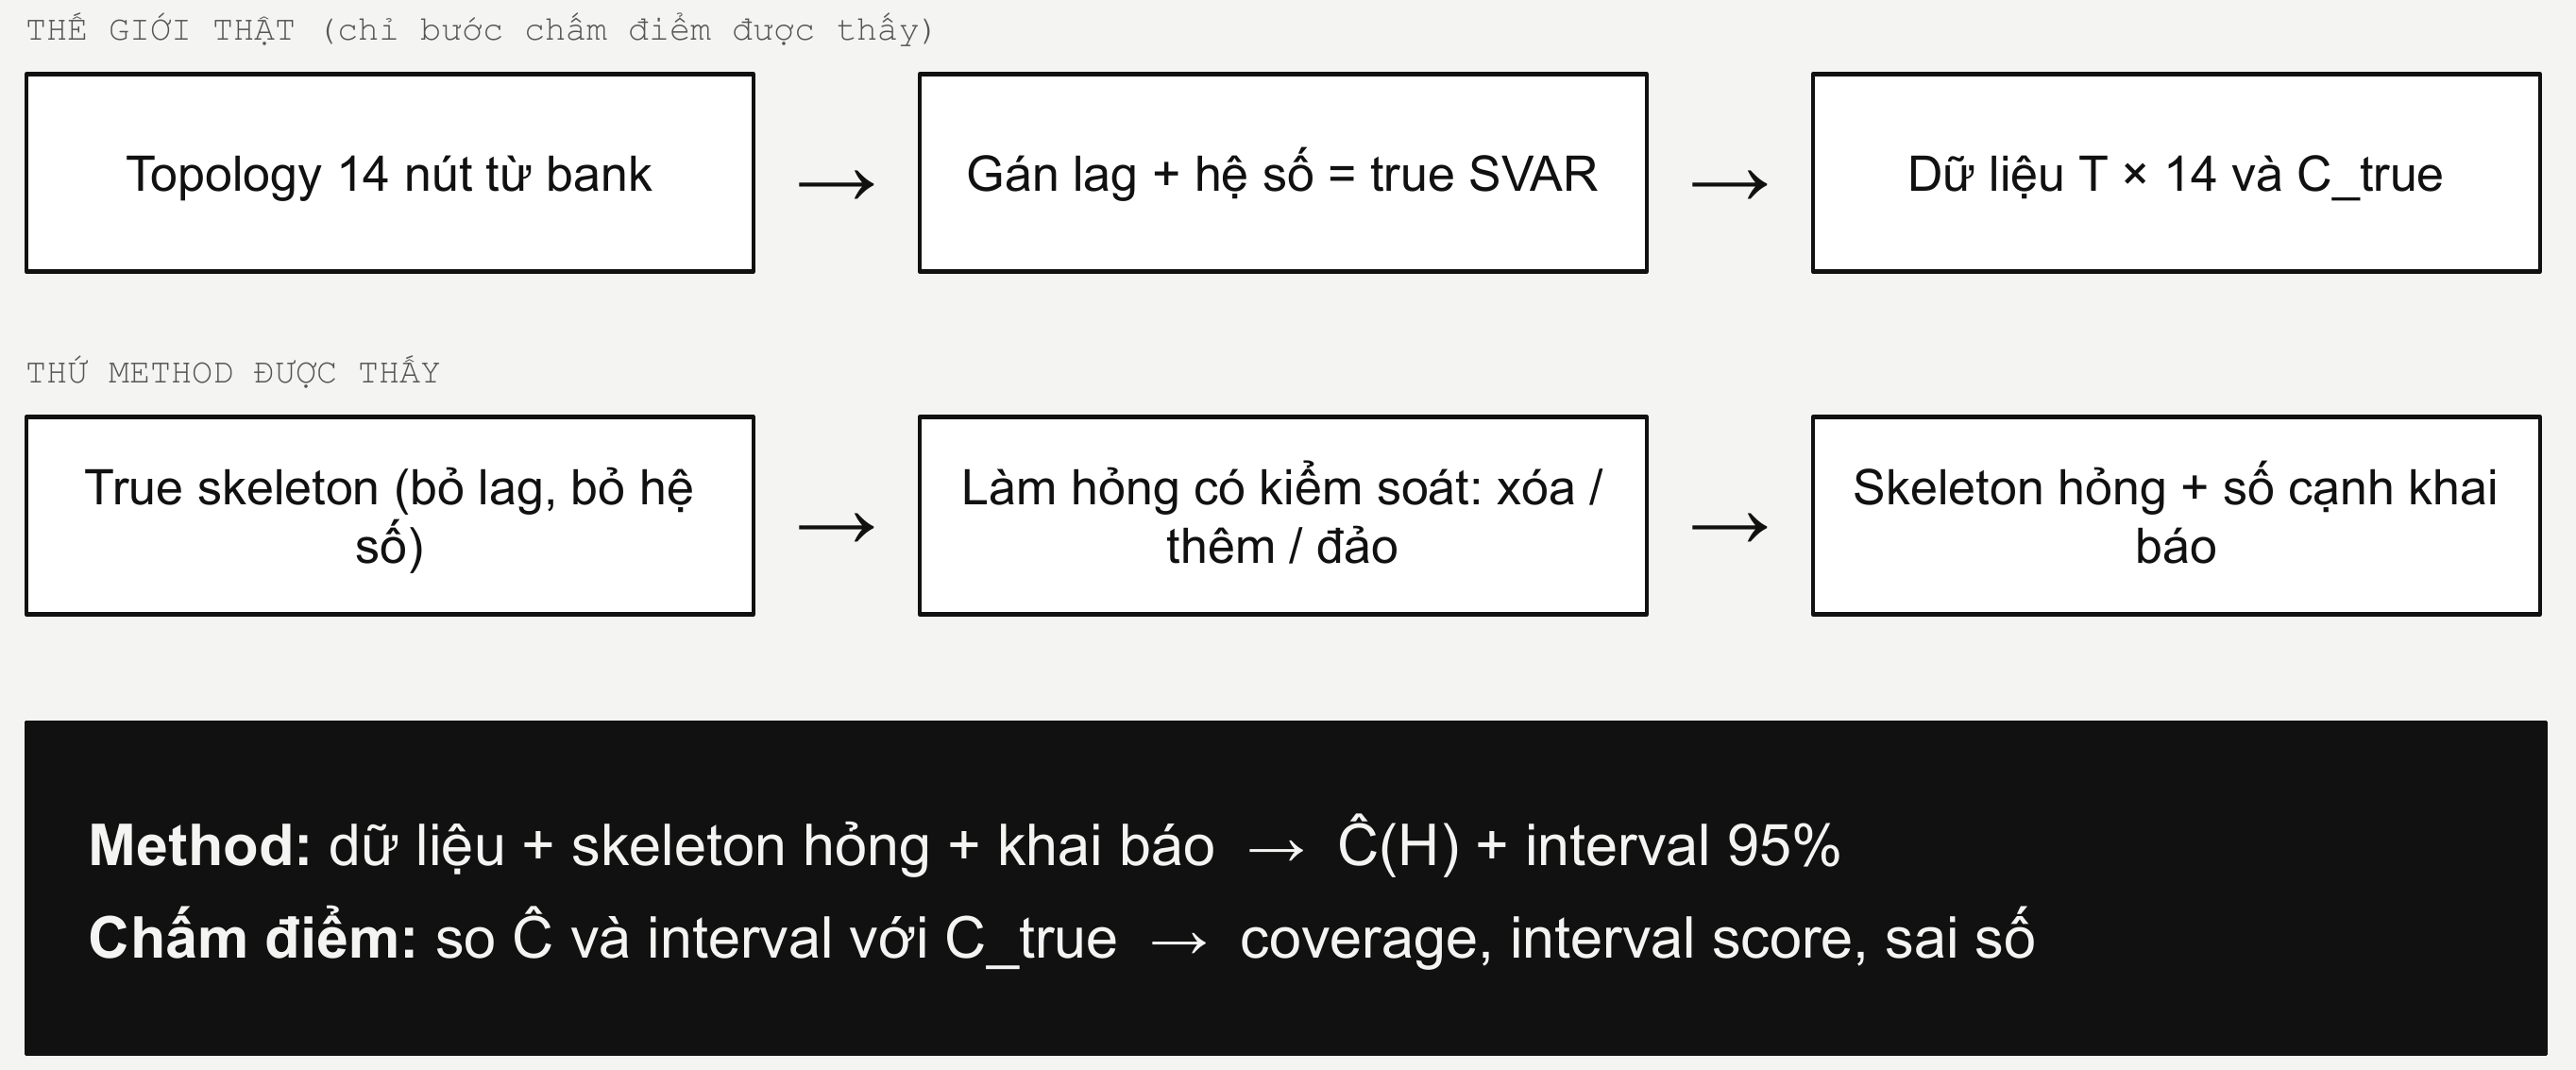
\includegraphics[width=\textwidth]{figures/quy_trinh_thuc_nghiem.png}
\caption{Quy trình một lượt thực nghiệm.}\label{fig:pipeline}
\end{figure}

Các bước cho mỗi bộ dữ liệu:
\begin{enumerate}
  \item Lấy một topology (đồ thị 14 nút, 21 cạnh).
  \item Gán lag và hệ số cho từng cạnh để được SVAR thật (mục~\ref{sec:generator}).
  \item Sinh $T\times14$ quan sát và tính $C(H)$ thật từ hệ số bằng \eqref{eq:irf}--\eqref{eq:cumulative}.
  \item Lấy skeleton thật (bỏ lag và hệ số), làm hỏng có kiểm soát (mục~\ref{sec:damage}) và ghi số cạnh hỏng làm khai báo.
  \item Đưa (dữ liệu, skeleton hỏng, khai báo) cho từng phương pháp; so $\hat C$ và khoảng tin cậy với $C(H)$ thật.
\end{enumerate}

\subsection{Sinh dữ liệu}\label{sec:generator}
Mỗi topology gồm 14 nút (7 ngân hàng, 3 biến vĩ mô, 4 chứng khoán) và 21 cạnh, thuộc hai họ đồ thị: Erdős--Rényi và scale-free có hub. Cấu trúc cạnh được sinh ngẫu nhiên.

\begin{table}[H]
\centering\small
\begin{tabularx}{\textwidth}{>{\raggedright\arraybackslash}p{4.3cm}Y}
\toprule
Thành phần & Cách rút\\
\midrule
Lag của mỗi cạnh & Cùng kỳ (lag 0) với xác suất $0.3$; còn lại ngẫu nhiên trong $\{1,\dots,p\}$, mặc định $p=2$ (khảo sát vùng dùng được thử $p\in\{1,2,4\}$)\\
Hệ số cạnh & $|b|\sim U(0.3,0.8)$, dấu ngẫu nhiên\\
Tự hồi quy & Hệ số lag 1 của mỗi nút $\sim U(0.2,0.6)$\\
Phương sai nhiễu & $\sigma_j^2\sim U(0.5,1.5)$ cho mỗi nút\\
Ổn định & Co phần lag đến khi bán kính phổ của ma trận companion $<0.9$\\
Burn-in & 200 quan sát đầu bị bỏ\\
Cỡ mẫu & $T\in\{40,80,150\}$ trong thực nghiệm chính; $T$ nhỏ tới $19$ trong khảo sát vùng dùng được\\
\bottomrule
\end{tabularx}
\caption{Tham số của bộ sinh dữ liệu.}
\end{table}

\subsection{Làm hỏng skeleton}\label{sec:damage}
Số cặp bị hỏng là $k=\lfloor \text{tỷ lệ}\times\text{cơ sở}+0.5\rfloor$, với cơ sở là số cạnh thật (21), hoặc, với đảo chiều, số cạnh cùng kỳ có thể đảo. Với 21 cạnh, tỷ lệ 20\% cho $k=4$ và 50\% cho $k=11$. Mỗi loại lỗi (thiếu, thừa, đảo) được thử ở hai mức 20\% và 50\%, cộng với trường hợp không hỏng: tổng cộng 7 cell. Phương pháp chỉ nhận cặp nối, chiều cạnh cùng kỳ và khai báo; không nhận danh sách cạnh hỏng, lag, hệ số hay $C(H)$ thật.

\subsection{Quy mô thực nghiệm}\label{sec:quymo}
Với mỗi cell, chúng tôi dùng một tập gồm 20 topology, mỗi topology 3 lần sinh dữ liệu độc lập, tổng cộng 60 bộ dữ liệu. Trên mỗi bộ dữ liệu, mỗi phương pháp chạy residual bootstrap $B=199$ lần để dựng khoảng tin cậy 95\% (phân vị 2.5\%--97.5\%). Thực nghiệm chính gồm 3 giá trị $T$, 7 cell và 60 bộ dữ liệu, tức $1260$ bộ cho mỗi phương pháp và khoảng $250$ nghìn lần fit.

Mỗi bộ có khoảng 30--40 cặp non-null, nên coverage của một cell được tính trên khoảng 2000 phép kiểm. Cặp mà phương pháp làm mất đường truyền ($\hat C=0$, khoảng $[0,0]$) được tính là trượt.

\subsection{Dữ liệu phát triển, hiệu chỉnh và kiểm chứng}
Chúng tôi dùng ba loại tập dữ liệu, mỗi loại gồm các topology khác nhau:
\begin{itemize}
  \item \textbf{Tập phát triển:} nơi thiết kế và thử phương pháp. Kết quả trên tập này mang tính thăm dò (exploratory) vì phương pháp có thể bị chỉnh theo chính nó.
  \item \textbf{Tập hiệu chỉnh:} chỉ dùng để chọn hệ số độ rộng (bước 6); không dùng để chấm điểm.
  \item \textbf{Tập kiểm chứng:} các tập topology sinh riêng bằng seed khác, chưa từng được dùng khi thiết kế phương pháp, không trùng cạnh với tập nào trước. Quy tắc kết luận được ghi trước khi chạy cùng giá trị băm (sha256) của code và cấu hình, và mỗi tập kiểm chứng chỉ được dùng một lần cho mỗi nhóm kết luận.
\end{itemize}
Các kết quả trong mục~\ref{sec:ket-qua} được gắn nhãn \emph{kiểm chứng} hoặc \emph{thăm dò} theo đúng nguồn dữ liệu này.

\subsection{Các phương pháp tham chiếu}\label{sec:baseline}
Bảng~\ref{tab:baselines} liệt kê các phương pháp tham chiếu cùng tên gọi trong tài liệu gốc. Phần sau mô tả từng phương pháp theo công trình gốc và cách áp dụng vào bài toán SVAR có skeleton cho sẵn. Hậu tố ``(cal)'' nghĩa là khoảng được nhân thêm hệ số độ rộng chọn theo $(T,\text{loại lỗi khai báo})$ trên tập hiệu chỉnh, theo đúng cách áp dụng cho \ours{}.

\begin{table}[H]
\centering\small
\begin{tabularx}{\textwidth}{>{\raggedright\arraybackslash}p{2.9cm}>{\raggedright\arraybackslash}p{4.3cm}Y}
\toprule
Ký hiệu & Tên trong công trình gốc & Nguồn\\
\midrule
Residual Bootstrap (RB) & Residual bootstrap cho IRF của VAR & \citet{kilian1998small}; \citet{efron1979bootstrap}\\
Oracle & RB trên đồ thị và lag thật & (mốc tham chiếu)\\
Inflate & Khoảng RB nới theo hệ số cố định & ---\\
Bagging & Bootstrap aggregation (bagging) & \citet{breiman1996bagging}\\
LP & Local projection; lag-augmented local projection & \citet{jorda2005estimation}; \citet{montiel2021local}\\
IDA & IDA (Intervention calculus when the DAG is Absent) & \citet{maathuis2009estimating}\\
BVAR-Minnesota & Bayesian VAR với Minnesota prior; chọn hyperparameter bằng marginal likelihood & \citet{doan1984forecasting}; \citet{litterman1986forecasting}; \citet{giannone2015prior}\\
PSel-Union & Post-selection inference for causal effects after causal discovery & \citet{chang2026post}\\
TLP & Targeted Local Projections; double bootstrap & \citet{nemtyrev2026targeted}\\
Full VAR & Unrestricted VAR & \citet{sims1980macroeconomics}\\
\bottomrule
\end{tabularx}
\caption{Các phương pháp tham chiếu và tên gọi trong tài liệu gốc.}\label{tab:baselines}
\end{table}

\paragraph{Residual Bootstrap và Oracle.}
Ước lượng SVAR đệ quy bằng OLS từng phương trình rồi dựng khoảng tin cậy cho IRF bằng cách rút phần dư có hoàn lại và fit lại \citep{kilian1998small,lutkepohl2005new,kilian2017structural}. Chúng tôi cắm skeleton vào mô hình \eqref{eq:svar}, chạy bootstrap $B=199$ lần và lấy phân vị 2.5\%--97.5\% (mục~\ref{sec:bootstrap}). Skeleton được giữ nguyên ở mọi lần chạy. Oracle là cùng quy trình trên đồ thị thật với lag đúng.

\paragraph{Inflate.}
Khoảng của RB được nới quanh trung điểm bởi hằng số $c$: $[m-c\,h,\;m+c\,h]$, với $m$ là trung điểm và $h$ là nửa độ rộng. $c$ được chọn theo từng $T$ trên tập hiệu chỉnh.

\paragraph{Bagging \citep{breiman1996bagging}.}
Bagging huấn luyện nhiều bản của một ước lượng trên các mẫu bootstrap rồi lấy trung bình để giảm phương sai. Ở đây mỗi lần chạy, skeleton bị xáo trộn ngẫu nhiên theo đúng loại và mức khai báo (thiếu: thêm $k$ cặp chưa có chiều với hạng tử lag; thừa: bỏ $k$ cặp; đảo: lật $k$ cạnh cùng kỳ mà không tạo chu trình), fit trên một mẫu bootstrap, và khoảng tin cậy là phân vị của các lần chạy.

\paragraph{LP: local projection \citep{jorda2005estimation,montiel2021local}.}
Local projection ước lượng $C_{ji}(H)$ bằng hồi quy trực tiếp $\sum_{h\le H}x_{j,t+h}$ lên $x_{i,t}$ và các biến điều khiển, không cần mô hình động đầy đủ. \citet{montiel2021local} chỉ ra rằng thêm một lag phụ vào biến điều khiển cho phép suy luận HAC thông thường mà không cần biết mức độ bền (persistence) của chuỗi. Ở đây hồi quy dùng $x_{i,t}$, các cha cùng kỳ của $i$ trong skeleton và lag $1..p{+}1$ của mọi nút, với sai số chuẩn Newey--West.

\paragraph{IDA \citep{maathuis2009estimating}.}
Khi đồ thị chỉ được biết đến lớp tương đương Markov (CPDAG), hiệu ứng nhân quả không xác định duy nhất. IDA ước lượng hiệu ứng theo từng đồ thị khả dĩ trong lớp rồi báo tập các giá trị. Ở đây chiều của skeleton chỉ được tin đến lớp tương đương; mỗi thành viên của lớp (tối đa 16) được fit như RB, khoảng tin cậy là union các khoảng và điểm ước lượng là trung bình.

\paragraph{BVAR-Minnesota \citep{doan1984forecasting,litterman1986forecasting,giannone2015prior}.}
Minnesota prior co hệ số của VAR về 0 với độ siết tăng theo lag; \citet{giannone2015prior} chọn hyperparameter bằng marginal likelihood. Ở đây mỗi phương trình có lag $1..p$ của mọi nút và các cha cùng kỳ của skeleton. Phương sai prior của hệ số lag $l$ của $x_i$ trong phương trình của $x_j$ là $(\lambda/l)^2\,s_j^2/s_i^2$, nhân thêm $\theta$ khi $i\ne j$ và cặp nằm ngoài skeleton, trong đó $s_i$ là độ lệch chuẩn phần dư của AR$(p)$ đơn biến. $(\lambda,\theta)$ được chọn trên lưới bằng marginal likelihood và khoảng tin cậy lấy từ các mẫu posterior.

\paragraph{PSel-Union \citep{chang2026post}.}
Công trình gốc xét suy luận nhân quả sau khi khám phá đồ thị: chạy thuật toán PC nhiều lần với test statistic bị thêm nhiễu ngẫu nhiên, giữ các đồ thị thu được và lấy union khoảng tin cậy; coverage đúng theo tiệm cận. Phương pháp gốc làm việc trên dữ liệu i.i.d. Gaussian, không có lag. Ở đây bước chọn được áp dụng trên VAR:
\begin{enumerate}
  \item Mỗi cặp được chọn khi z-score Granger (hai chiều) hoặc z-score tương quan riêng của phần dư vượt $1.96$. Mỗi lần chọn cộng nhiễu $\mathcal N(0,\tau^2)$ vào mọi z-score; lặp 100 lần.
  \item Giữ đồ thị không nhiễu và các đồ thị nhiễu xuất hiện nhiều nhất, tối đa $16$.
  \item Cặp được chọn mà skeleton chưa có chiều được fit theo cả hai chiều với hạng tử cùng kỳ.
  \item Mỗi thành viên chạy đủ $199$ lần bootstrap; khoảng tin cậy là union (min của cận dưới, max của cận trên) qua mọi thành viên.
\end{enumerate}
Phương pháp không đọc mức hỏng khai báo. Mỗi lần gọi dùng khoảng $6368$ lần bootstrap, gấp $32$ lần \ours{}. Chúng tôi báo cáo bản có và không có hiệu chỉnh độ rộng (PSel-Union, PSel-Union (cal)) cùng một biến thể rút gọn với tối đa $16$ đồ thị và ít lần bootstrap hơn (PSel).

\paragraph{TLP: Targeted Local Projections \citep{nemtyrev2026targeted}.}
TLP co ước lượng LP về một mô hình có cấu trúc (VAR) làm mục tiêu, theo trọng số tối ưu MSE:
\begin{equation}
\hat\beta^{\mathrm{TLP}}_h=v_h\,\hat\beta^{\mathrm{LP}}_h+(1-v_h)\,\hat\beta^{\mathrm{VAR}}_h,\qquad
v_h=\max\Bigl[1-\frac{\Sigma^{\mathrm{LP}}_h-\Sigma^{\mathrm{COV}}_h}{T(\hat\beta^{\mathrm{LP}}_h-\hat\beta^{\mathrm{VAR}}_h)^2},\,0\Bigr].
\end{equation}
Suy luận dùng double bootstrap hai tầng: tầng một bootstrap phần dư của VAR rút gọn, tầng hai lặp lại thủ tục trên từng mẫu của tầng một. Ở đây mô hình mục tiêu là RB trên skeleton cho sẵn, nên các ràng buộc zero của skeleton đóng vai sai lệch cục bộ khi skeleton hỏng. TLP (cal) dùng bootstrap một tầng kiểu VAR-sieve; TLP-DB dùng double bootstrap với số lag LP $p=3$ và $200\times100$ lần bootstrap.

\paragraph{Full VAR \citep{sims1980macroeconomics}.}
VAR không ràng buộc với lag của mọi nút trong mọi phương trình, cộng các cạnh cùng kỳ của skeleton; không bổ sung cạnh, không chọn lọc lag. Đây là cách mở mọi lag mà \ours{} tránh.

\subsection{Chi phí tính toán}
Bảng~\ref{tab:budget} so sánh số lần bootstrap và thời gian mỗi lần gọi. PSel-Union (cal), phương pháp tham chiếu mạnh nhất, dùng gấp $32$ lần số lần bootstrap và $6.6$--$7.9$ lần thời gian của \ours{}.
\begin{table}[H]
\centering\small
\begin{tabularx}{\textwidth}{lYrr}
\toprule
Phương pháp & Số lần bootstrap mỗi lần gọi & s/gọi, $T{=}80$ & $T{=}150$\\
\midrule
\ours{} & 199 (chọn lại lag mỗi lần) & 1.27 & 1.44\\
PSel-Union (cal) & 16 đồ thị, 32 thành viên $\times$ 199, trung bình 6368 & 8.34 & 11.42\\
PSel & $\le16$ đồ thị $\times\max(10,199\!\div\!\#)$ & 0.28 & 0.36\\
Full VAR (cal) & 199 & 0.51 & 0.61\\
TLP (cal) & 199 (VAR-sieve một tầng) & 0.31 & 0.40\\
TLP-DB & $200\times100$ & 5.14 & 6.03\\
BVAR-Minnesota (cal) & 199 mẫu posterior & 0.09 & 0.08\\
\bottomrule
\end{tabularx}
\caption{Chi phí tính toán (median của 6 lần gọi trên tập phát triển).}\label{tab:budget}
\end{table}

\subsection{Chỉ số đánh giá}\label{sec:metric}
\begin{description}
  \item[Coverage] tỷ lệ khoảng tin cậy chứa giá trị thật; mục tiêu khoảng $0.95$.
  \item[Độ rộng] $u-\ell$. Hẹp chỉ có ý nghĩa khi coverage đạt.
  \item[Interval score (IS)] \citep{gneiting2007strictly}. Với khoảng $[\ell,u]$ mức $1-\alpha$ và giá trị thật $c$:
  \begin{equation}
  \IS_\alpha(\ell,u;c)=(u-\ell)+\frac{2}{\alpha}(\ell-c)\,\mathbf 1\{c<\ell\}+\frac{2}{\alpha}(c-u)\,\mathbf 1\{c>u\}.
  \end{equation}
  Với $\alpha=0.05$, hệ số phạt là $2/\alpha=40$. IS càng thấp càng tốt và gộp cả độ rộng lẫn việc trượt. Ví dụ với $c=1.0$: khoảng $[0.8,1.2]$ có $\IS=0.4$; khoảng $[1.1,1.2]$ trượt $0.1$ có $\IS=0.1+40\times0.1=4.1$; khoảng $[-5,7]$ chứa $c$ nhưng quá rộng có $\IS=12$. IS của một lượt chạy là trung bình trên các cặp non-null.
  \item[Sai số cường độ] $|\hat C-C|$, tuyệt đối và tương đối.
  \item[Sai số lag] lệch mean lag và việc peak lag có đúng không.
\end{description}

\subsection{Phương pháp thống kê}
So sánh giữa hai phương pháp dùng hiệu IS trên cùng bộ dữ liệu. Vì các bộ dữ liệu cùng topology không độc lập, khoảng tin cậy 95\% của hiệu được tính bằng cluster bootstrap, resample cả topology; một cell chỉ được tính khi có ít nhất 8 cụm topology. Các so sánh trong cùng một họ được hiệu chỉnh đa kiểm định bằng phương pháp Holm \citep{holm1979simple} ở mức 0.05.
